\section{Astrodynamics \& control tool development}
\label{ch:astrocontrol}
In this chapter the development of a tool for astrodynamics and control is described. The tool calculates the trajectory of the spacecraft for varying initial conditions and aerodynamic properties. With the information extracted from this tool requirements**maybe requirements is not the right word** for the control systems can be determined. Based on these requirements the different control systems available for the different concepts (which are presented in chapter \ref{ch:options}) can be weighed off in a trade-off in chapter \ref{ch:tradeoff}.

In this chapter first the purpose of the tool will be explained in section \ref{sec:astropurpose}. In sections \ref{sec:astrogov} and \ref{sec:astrowp} working principles of the tool are explained and the equations the tool is based on are presented. To ensure the tool calculates what it is supposed to calculate and to ensure this happens accurately enough in section \ref{sec:astrovv} the verification and validation of the tool is done. In section \ref{sec:astroref} performance of current day control systems are investigated. This performance is compared to the calculated needed performance to come to a conclusion in section \ref{sec:astrores}. Section \ref{sec:astrores} also presents some other results of the tool which are used as input for tools calculating i.e. structural mass.

\subsection{Purpose of tool development}
\label{sec:astropurpose}
The purpose of developing a tool to calculate the trajectory of the spacecraft during entry is firstly to know the trajectory given the characteristics of the spacecraft. Secondly, calculating trajectories for varying input, for the different concepts and different control systems, this tool can also give an insight in which concepts have the characteristics needed for a successful entry.

The tool has been developed in-house as no existing tool that suits our purpose and is publicly available has been found.

More specifically the tool is used here to determine the required Aerodynamic characteristics to create an acceptable window of entry. Or in other words: What accuracy of the initial conditions is needed to, with a certain shape and control, get the required accuracy at the final position. Taking into account the different shapes the goal of this tool is to investigate the need for \& effect of control on the trajectory of the spacecraft. 

\subsection{Governing equations}
\label{sec:astrogov}
***intro***\\
***Kepler for hyperbolic: Vis-Viva, polar expression of hyperbola, tangent to hyperbola)***\\
***Forces give accelerations: like in baseline + Jerk***\\
***Kepler for elliptic: symmetry***\\


\subsubsection{Atmospheric model}
\begin{figure}[h]
	\centering
	\begin{subfigure}{0.45\textwidth}
	\centering
	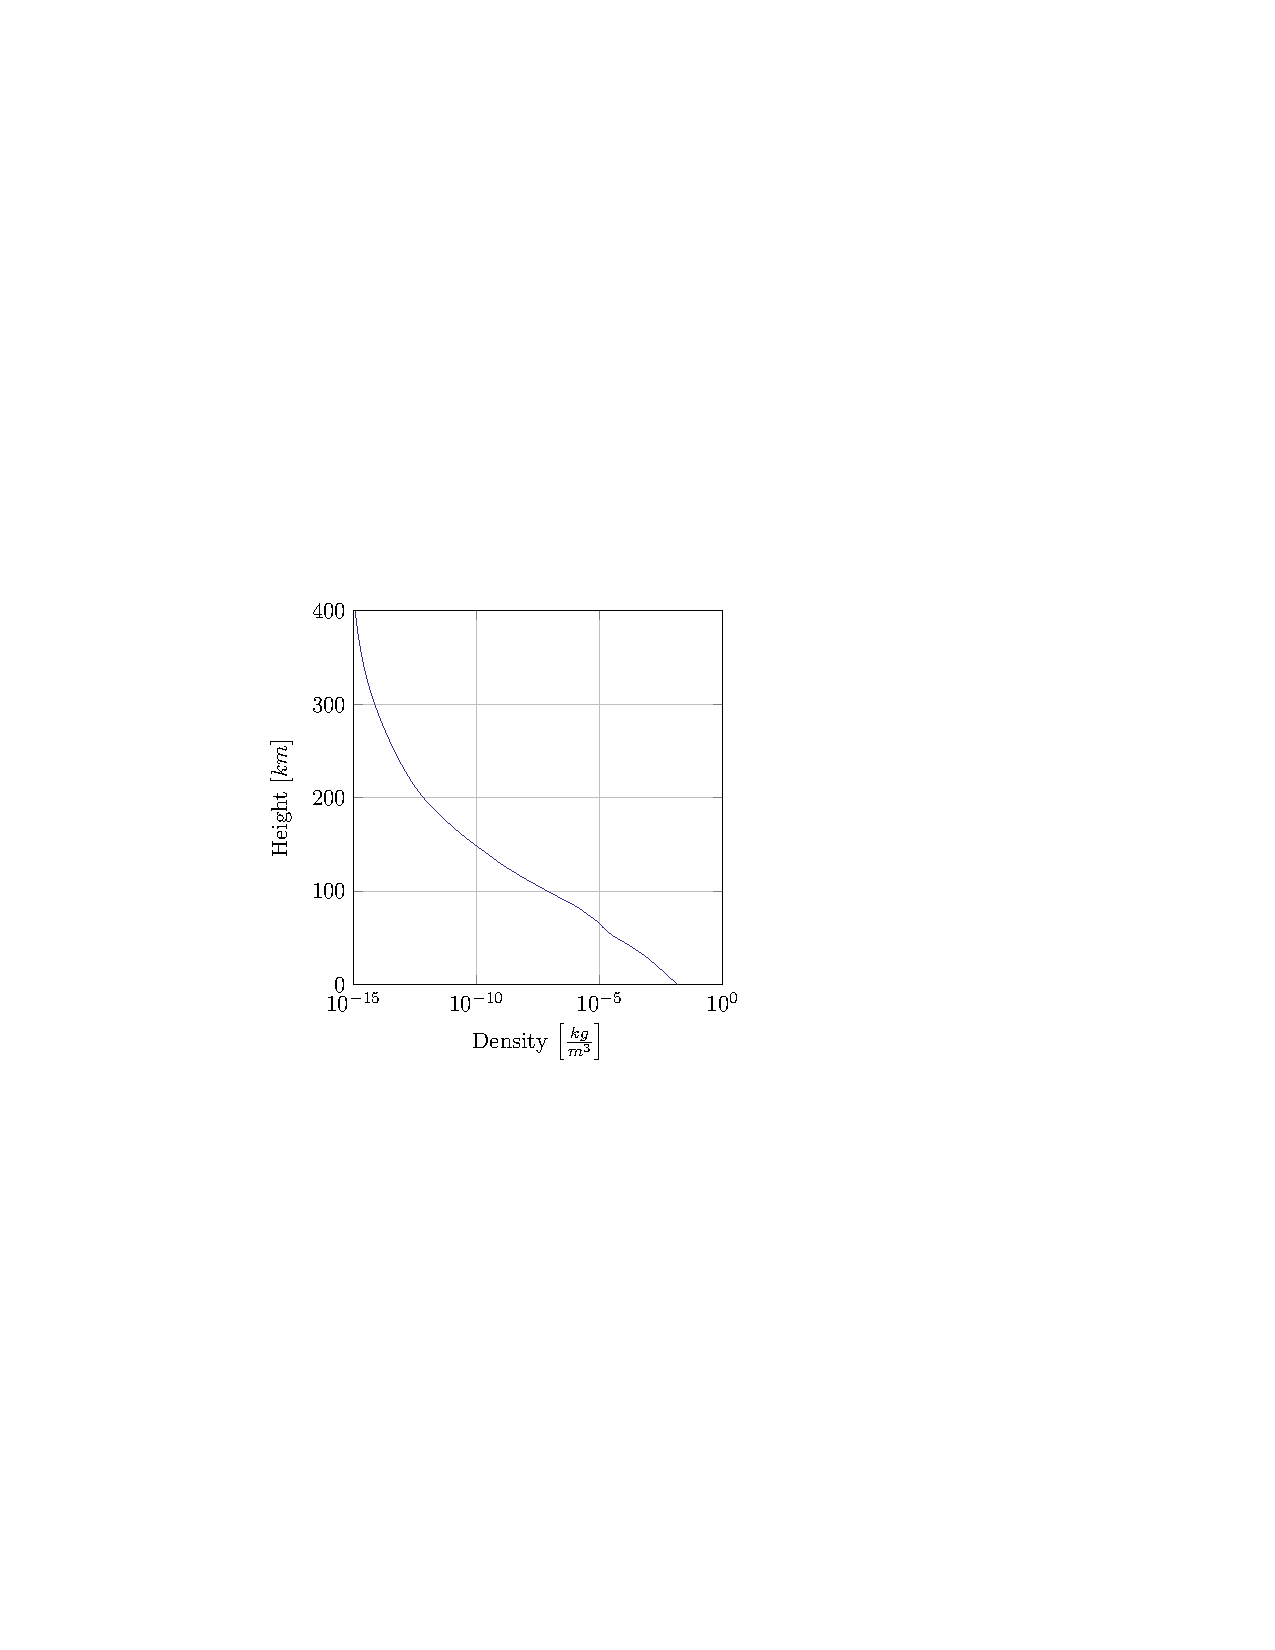
\includegraphics[trim={4cm 9.8cm 5cm 10cm},clip,width=1.3\textwidth]{Figure/atmos_model/density.pdf}
	\caption{The atmospheric density} 
	\label{fig:atmos_height_rho}
	\end{subfigure}
	\begin{subfigure}{0.45\textwidth}
	\centering
	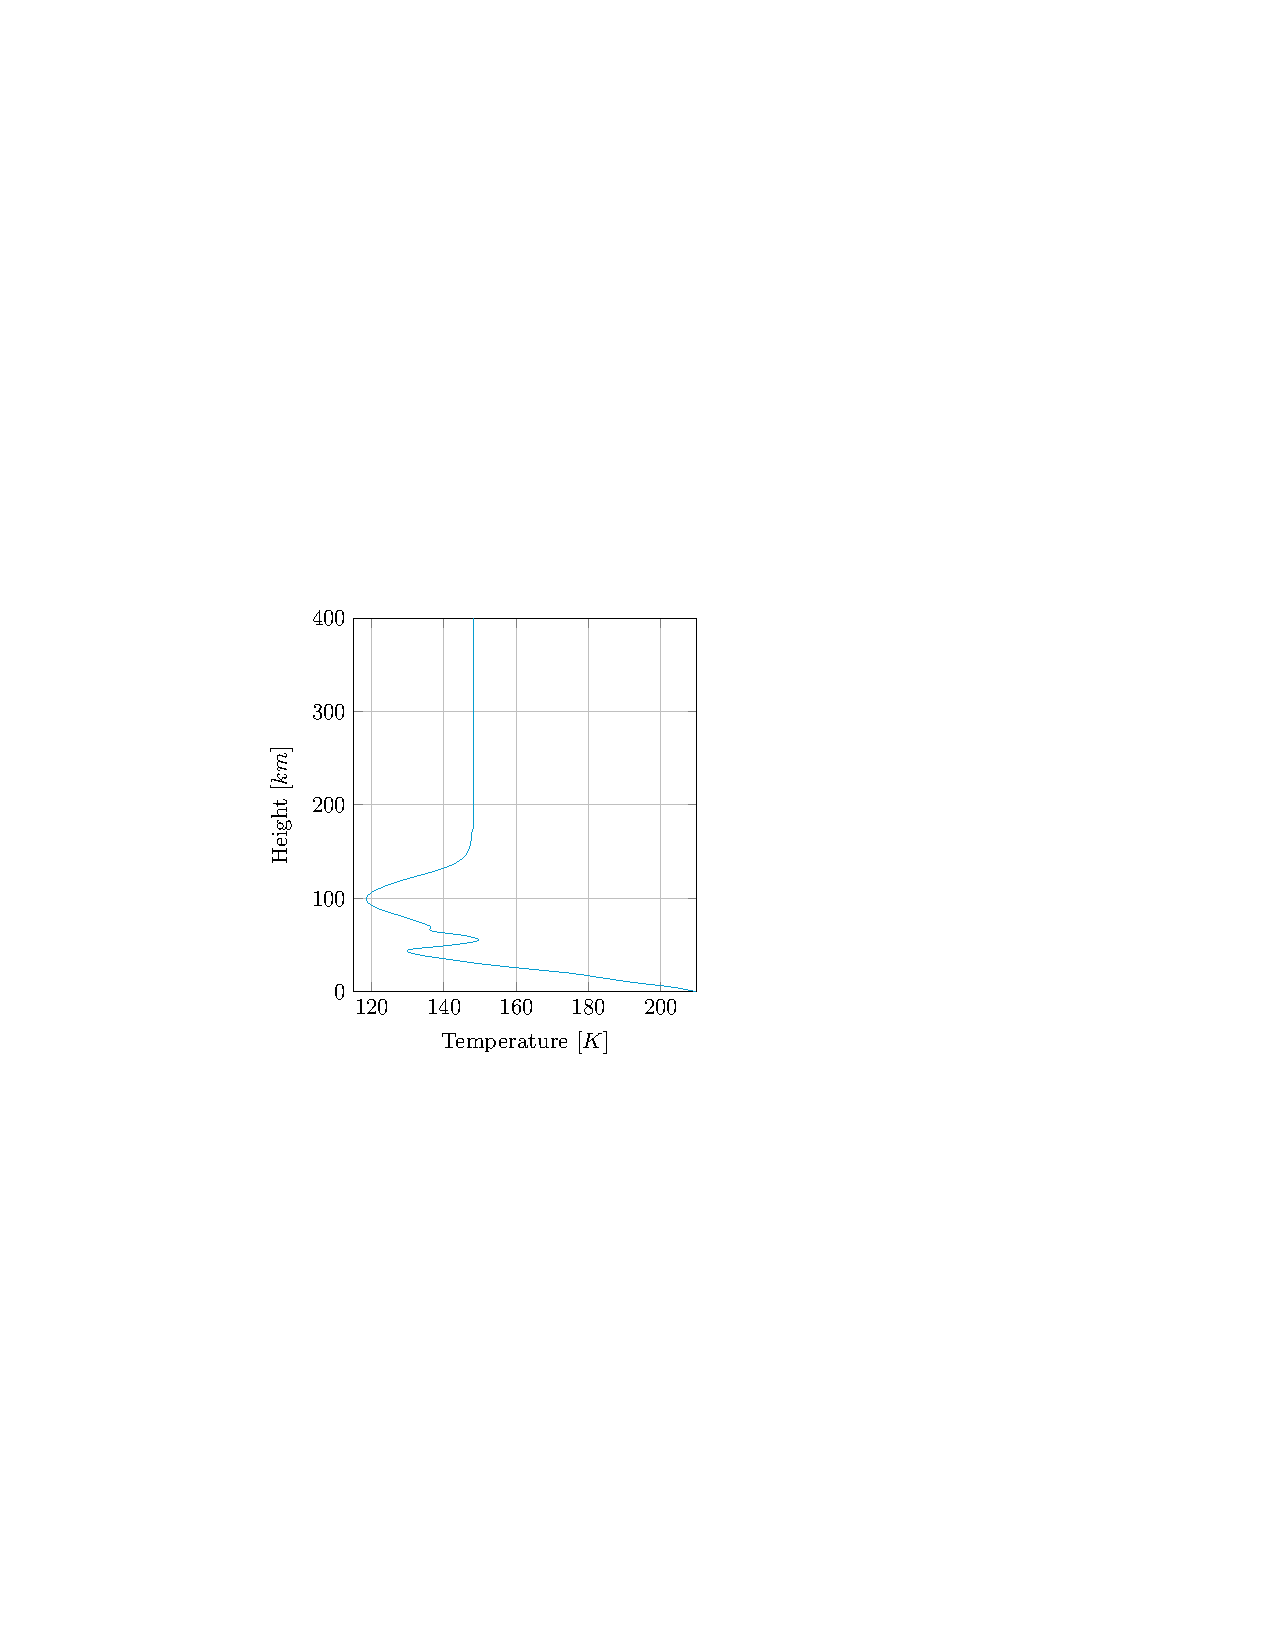
\includegraphics[trim={4cm 9.8cm 5cm 10cm},clip,width=1.3\textwidth]{Figure/atmos_model/temperature.pdf}
	\caption{The atmospheric temperature}
	\label{fig:atmos_height_T}
	\end{subfigure}
	\caption{The atmospheric properties for different heights}
	\label{fig:atmos_height}
\end{figure}

\begin{figure}[h]
	\centering
	\begin{subfigure}{0.9\textwidth}
	\centering
	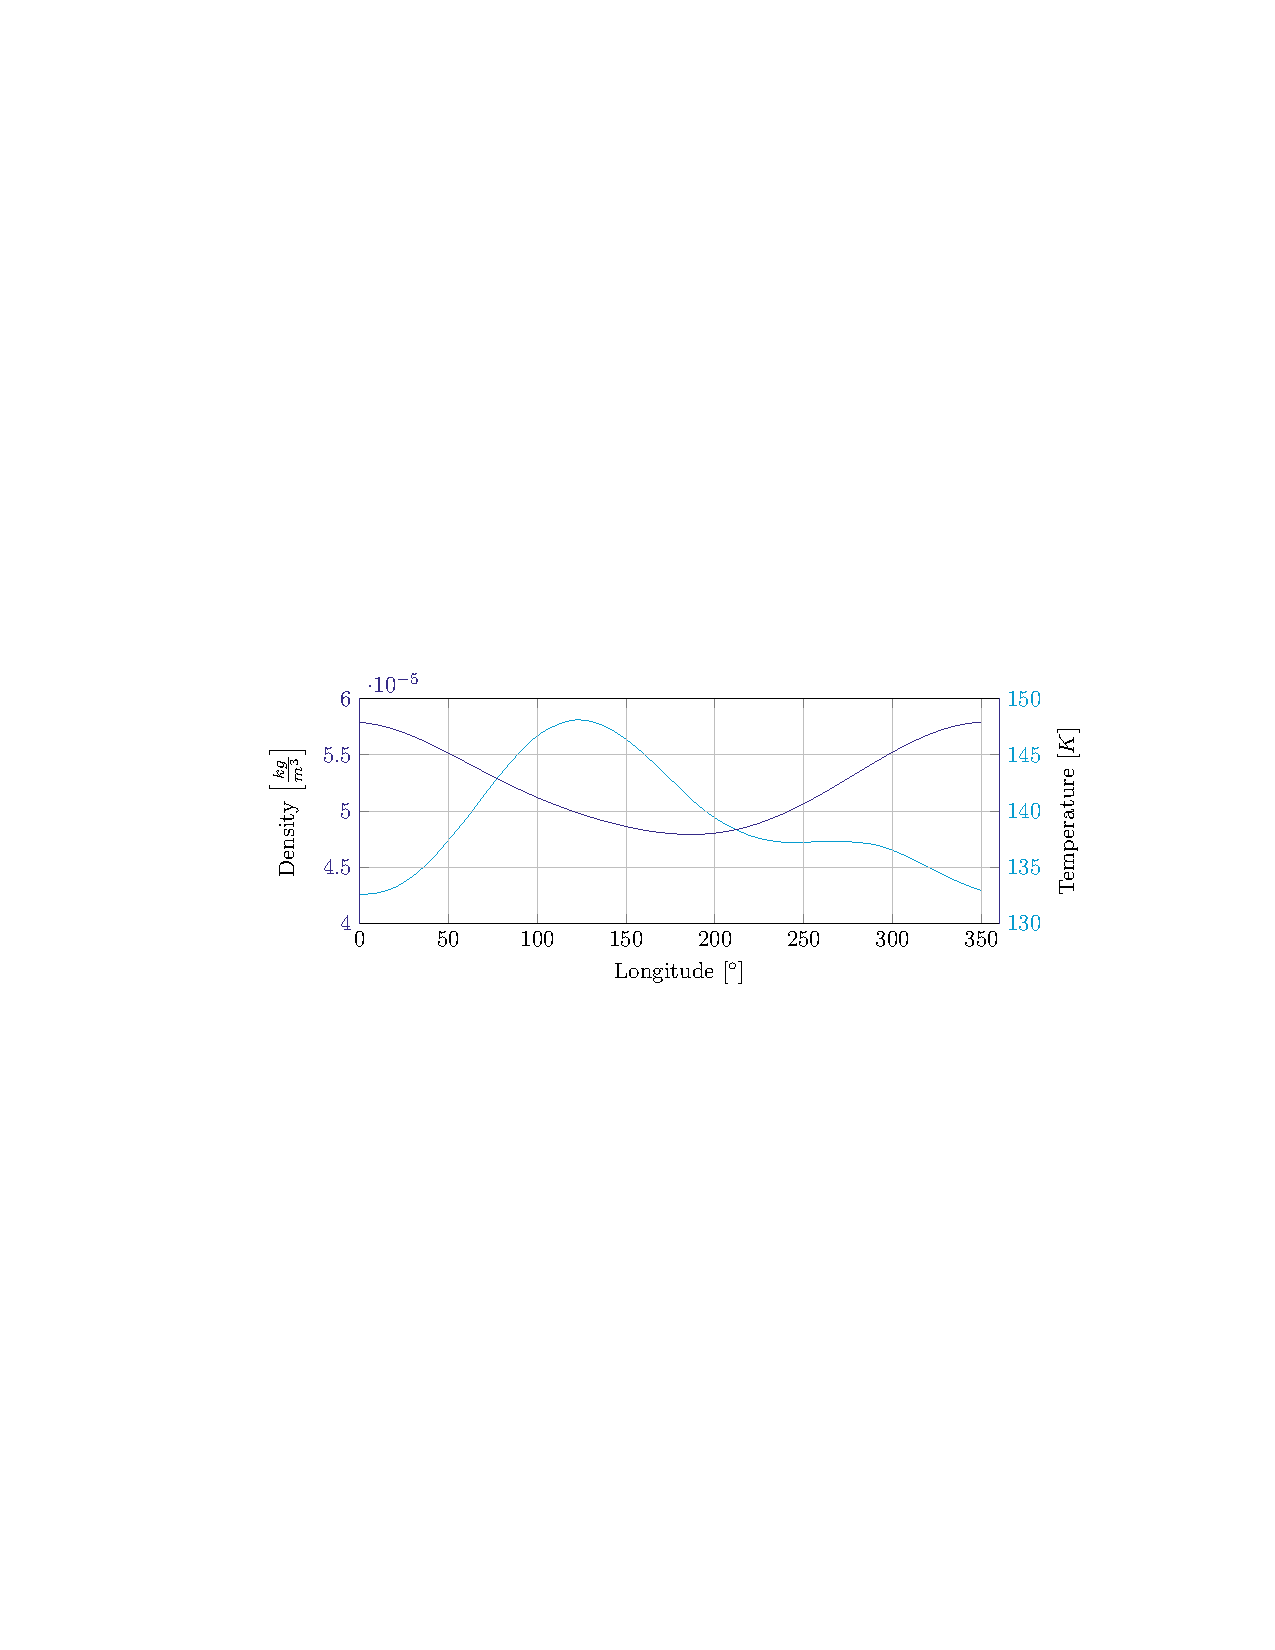
\includegraphics[trim={4.25cm 11cm 3.2cm 11cm},clip,width=0.9\textwidth]{Figure/atmos_model/lon_50.pdf}
	\caption{The atmospheric properties at $50$ $\left[km\right]$} 
	\label{fig:atmos_lon_50}
	\end{subfigure}
	\begin{subfigure}{0.9\textwidth}
	\centering
	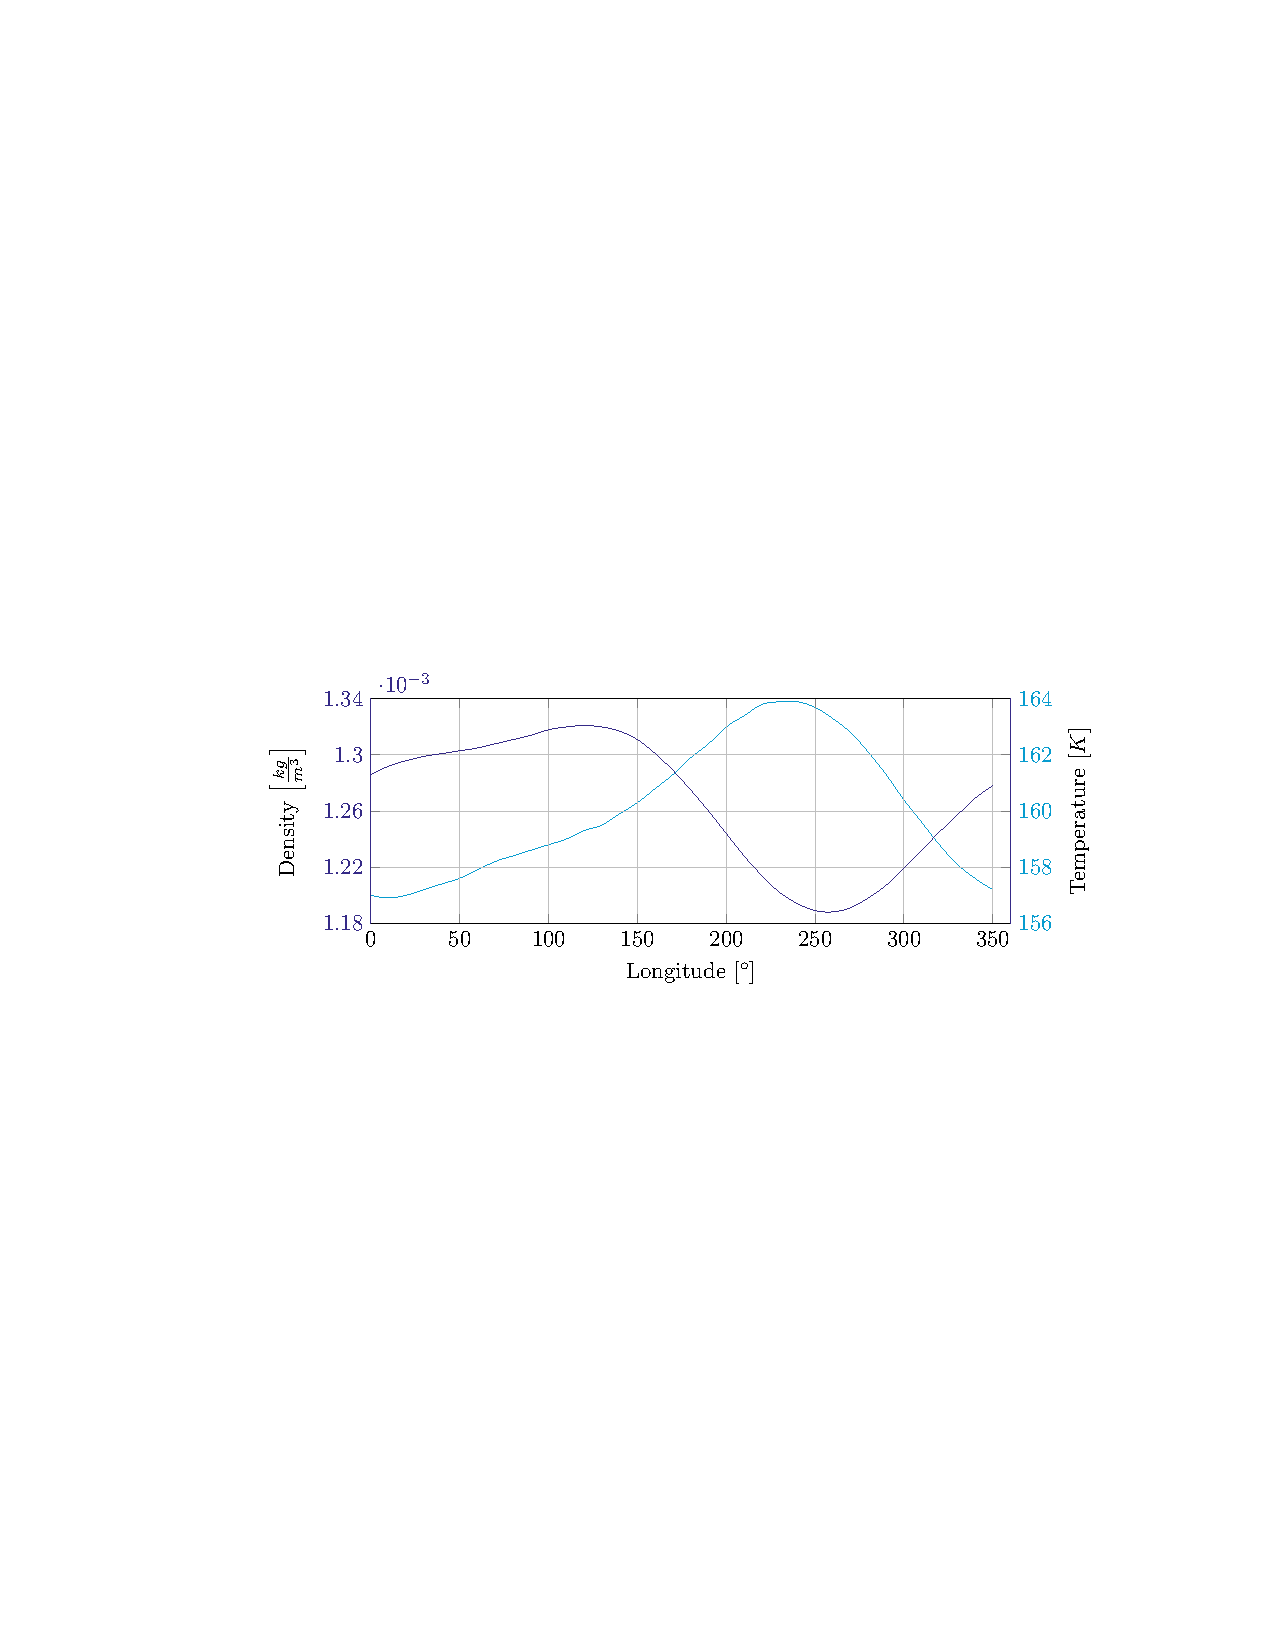
\includegraphics[trim={4.5cm 11cm 3.1cm 11cm},clip,width=0.9\textwidth]{Figure/atmos_model/lon_25.pdf}
	\caption{The atmospheric properties at $25$ $\left[km\right]$} 
	\label{fig:atmos_lon_25}
	\end{subfigure}
	\caption{The atmospheric properties for different heights}
	\label{fig:atmos_lon}
\end{figure}

\subsection{Working principles of the tool}
\label{sec:astrowp}
The tool is able to calculate the trajectory of the spacecraft and a range of important parameters at each moment in time. These parameters are among others: Acceleration (\gls{sym:acc}), dynamic pressure (\gls{sym:q}), speed (\gls{sym:Vv}) and Mach number (\gls{sym:M}). In order to calculate this the tool takes geometric and aerodynamic properties of the spacecraft and some initial conditions as input.

***Flowchart + very short explanation***\\

\subsection{Verification \& validation}
\label{sec:astrovv}
***intro***\\
***sensitivity analysis: very sensitive to initial location, thus for now assumed initial location closer***\\
***discretisation error: error for different dt***\\
***Compare numerical results with Kepler, should be the same for rho=0***\\
***Validation through checking if output values are approximately the same as reference cases (peak dynamic pressure)***\\

\subsection{Performance of control systems}
 \label{sec:astroref}
***intro***\\
***Moment or dalpha/dt that control systems (cg offset, thrusters, control surfaces) can create***\\
***Weight estimate of each control system (per concept if needed)***\\

\subsection{Results \& Conclusions}
\label{sec:astrores}
***intro***\\
***Plot of a trajectory***\\
***Plots of output variables for that particular trajectory***\\
***Results of needed CLmax, dalpha/dt, dCL/dalpha***\\
***Conclusion on which control system (implemented in which concept) can perform as such***\\
***Conclusion on weight the control systems will bring along***\\
***State values for in trade-off matrix***\\